\subsection{Recovery Mechanism}
\label{sec:recovery}

As described in Section~\ref{fault_tolerance:sec:design}, recovering from a
failure consists of two central actions: write recovery and read recovery. In
the case of \themis, write recovery involves recovering partitions on any
intermediate disk that failed, while read recovery involves re-generating
missing pieces of partitions that a failed node should have produced, but
didn't. When a job fails, \themis will recover it by running a \emph{recovery
  job}, which is treated like a normal MapReduce job but is dedicated to
recovery.

\begin{figure}
  \centering
  \begin{subfigure}[t]{\columnwidth}
    \centering
    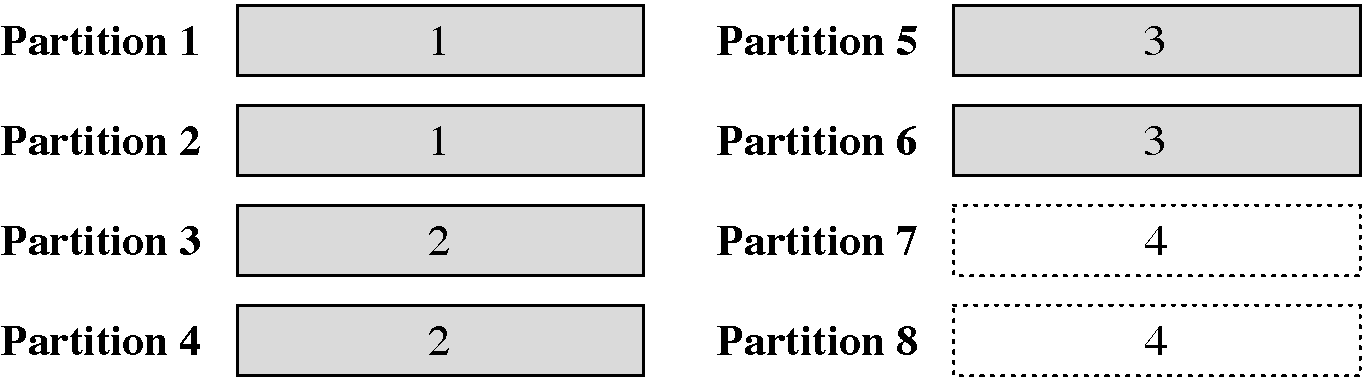
\includegraphics[width=\textwidth]{fault_tolerance/figures/disk_failure_before_recovery}
    \caption{\label{fig:disk_fail_before} The state of the job's intermediate
      partitions after the failure of disk 4. All intermediate partitions
      stored on disk 4 has been lost.}
  \end{subfigure}\hspace{0.05\textwidth}
  \begin{subfigure}[t]{\columnwidth}
    \centering
    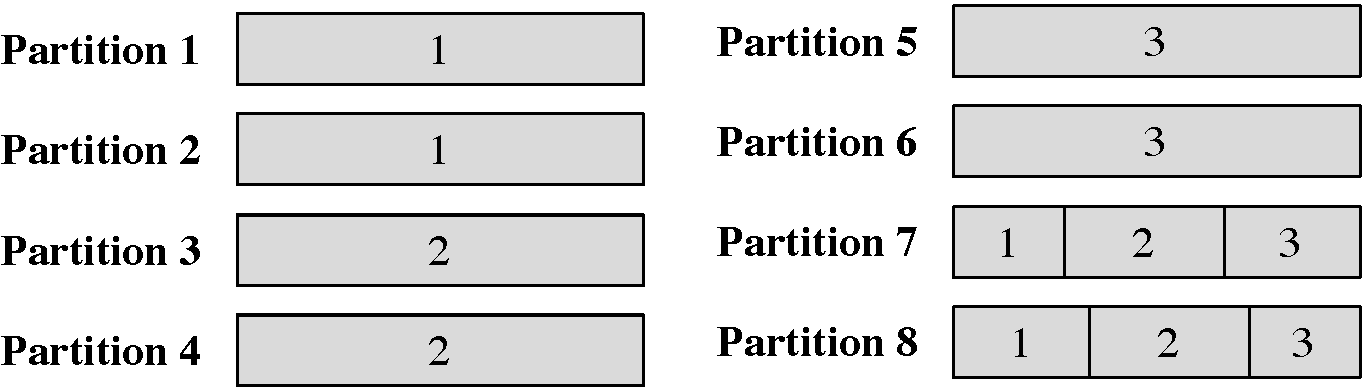
\includegraphics[width=\textwidth]{fault_tolerance/figures/disk_failure_after_recovery}
    \caption{\label{fig:disk_fail_after} The state of the job's intermediate
      partitions after recovery from the disk failure. Intermediate data for
      the partitions on disk 4 have spread across disks 1 through 3.}
  \end{subfigure}
  \caption{\label{fig:disk_fail} Illustrative example of disk failure and
    recovery in a two-node cluster with two intermediate disks per node and
    eight intermediate partitions. The rectangles
    representing each partition are labeled with the disk or disks on which
    data for that partition is stored.}
\end{figure}

Before we explore the technical details of the implementation, consider the
following illustrative example. Suppose that \themis is running on a two-node
cluster with two intermediate disks each, storing a total of eight intermediate
partitions for a particular job. In Figure~\ref{fig:disk_fail_before}, disk 4
in this cluster has failed during phase one, causing the loss of partitions 7
and 8. Figure~\ref{fig:disk_fail_after} shows the state of the intermediate
partitions at the end of phase one of the recovery job, when the data for
partitions 7 and 8 has been recovered.

Note that the recovered data for partitions 7 and 8 is spread across all the
remaining disks roughly evenly; this is highly desirable because it allows as
many disks as possible to participate in phase two of the recovery job. It
should also be noted that after the failure of disk 4 in phase one, phase two
can be run to completion on partitions 1 through 6 without waiting for the
recovery job to recover the other partitions.

\begin{figure}[t]
  \centering
  \begin{subfigure}[t]{\columnwidth}
    \centering
    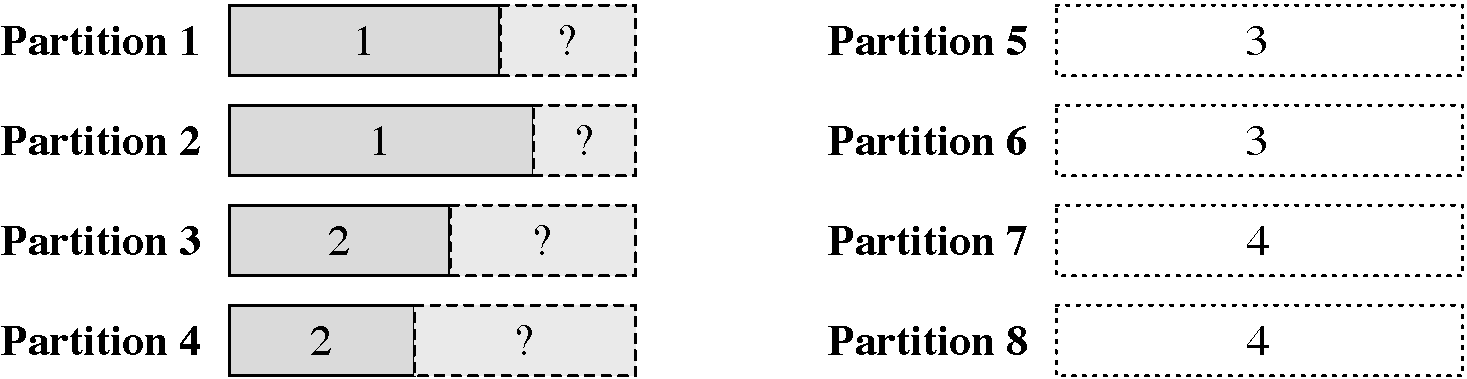
\includegraphics[width=\textwidth]{fault_tolerance/figures/node_failure_before_recovery}
    \caption{\label{fig:node_fail_before} The state of the job's intermediate
      partitions after the failure of node 2. All intermediate data for disks 3
      and 4 has been lost, and some data for the remaining partitions may not
      have been generated.}
  \end{subfigure}\hspace{0.05\textwidth}
  \begin{subfigure}[t]{\columnwidth}
    \centering
    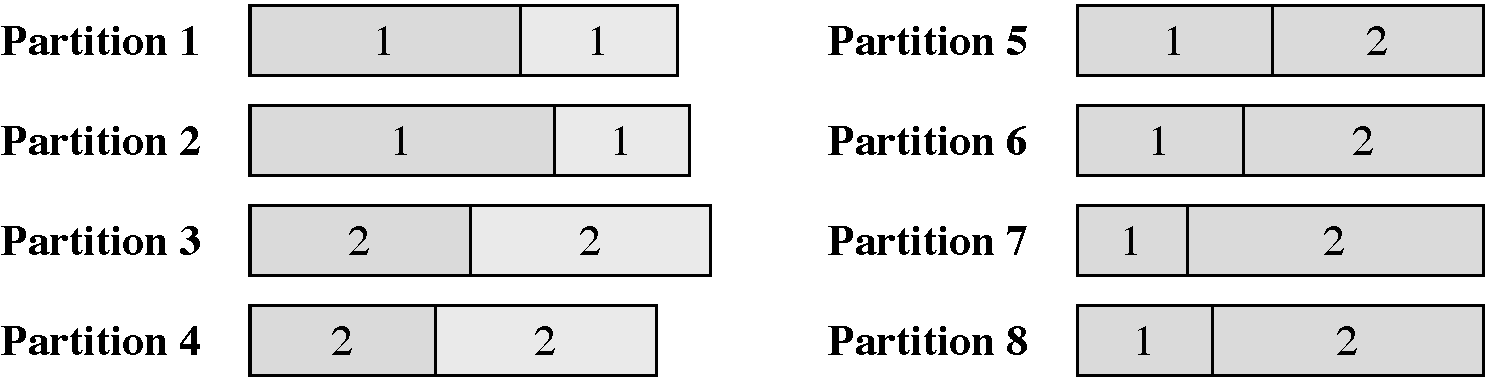
\includegraphics[width=\textwidth]{fault_tolerance/figures/node_failure_after_recovery}
    \caption{\label{fig:node_fail_after} The state of the job's intermediate
      partitions after recovery from the node failure. Intermediate data for
      the partitions on disks 3 and 4 have spread across disks 1 and 2, and
      data that should have been produced by node 2 has been added to node 1's
      partitions (although there may be duplicates).}
  \end{subfigure}
  \caption{\label{fig:node_fail} Illustrative example of node failure and
    recovery in a two-node cluster with two intermediate disks per node and
    eight intermediate partitions. A '?' indicates that it is unknown
    whether the data has been lost or not.}
\end{figure}

Figure~\ref{fig:node_fail_before} shows the same cluster after experiencing a
failure of an entire node. Not only have partitions 5 through 8 been lost, but
the remaining partitions are incomplete because the node did not finish
producing intermediate data for those partitions before it failed. Once phase
one of the recovery job has completed in Figure~\ref{fig:node_fail_after},
write recovery has spread the lost data from partitions 5 through 8 across
disks 1 and 2, while read recovery has ensured that every record that belongs
in partitions 1 through 4 has been written at least once.

\begin{table*}[t]
  \centering
  \caption{\label{table:failure_response} Table summarizing \themis' response
    to various kinds of failures at different points in the job.}
  \resizebox{\columnwidth}{!}{
  \begin{tabular}{|c|c|c|c|c|}
    \hline
    \textbf{Phase} & \textbf{Failure} & \textbf{Write Recovery} & \textbf{Read Recovery} & \textbf{Run Subsequent Phases?} \\
    \hline
    Zero (Sample) & Any & None & None & Yes \\
    One (Map + Shuffle) & Disk & Failed disk's partitions & None & Yes \\
    One (Map + Shuffle) & Node & All node's disks' partitions & Node's input files & No \\
    Two (Sort + Reduce) & Disk & Failed disk's partitions & None & Yes \\
    Two (Sort + Reduce) & Node & All node's disks' partitions & None & Yes \\
    \hline
  \end{tabular}
}
\end{table*}

In contrast to disk failure, phase two cannot be run after a node failure in
phase one because some intermediate partitions may not be complete.

If a disk or node fails in phase two, write recovery must be performed to
restore the intermediate data that was lost in the failure, but no read
recovery must be performed. Since phase zero is optional and does not produce
any output aside from a partition function, any failure during phase zero
simply requires re-executing it.

The responses to various kinds of failure in each of \themis' stages is
summarized in Table~\ref{table:failure_response}.

In the following sections, we will describe the mechanisms behind both write
and read recovery.

\subsubsection{Write Recovery}

To perform write recovery, the recovery job must re-map the failed job's input,
discarding any records that were not stored on the intermediate disks that
failed. To do this, the recovery job wraps its partition function in a
\emph{record filter}. This filter is applied to each record before it is passed
to the partition function. Abstractly, a record filter is a function that takes
a record as input and returns either ``accept'' or ``reject''. The filter
accepts a record if the record belongs to one of the partitions being
recovered, and rejects it otherwise.

In practice, \themis accomplishes record filtering in one of two ways. If the
failed job was using a user-defined partition function, the record filter
applies the failed job's partition function to the record. If the resulting
partition number is outside the range of partitions to be recovered, the filter
rejects the record.

If the original job is using a partition function generated by phase zero, the
record filter stores a set of boundary key ranges, one per contiguous range of
partitions being recovered. The complete list of boundary keys for each
partition is stored on distributed storage at the end of phase zero, and the
filter retrieves the appropriate boundary keys when it is constructed.

When an intermediate record is emitted by the \map function, the filter first
compares each intermediate record's key to the boundaries of each of its
ranges; if the record is within any of the filter's ranges, the filter
accepts the record.

In order to speed recovery by writing to as many disks in parallel as possible,
the intermediate data being recovered is spread across the cluster's remaining
intermediate disks. This is done by running phase zero during the recovery job
on a filtered sample of the input data, which generates a partition function
that spreads data in the filtered partition ranges evenly throughout the cluster.

At the end of phase one of the recovery job, any partitions that were
completely lost during a failure have been reconstituted and spread across the
cluster's remaining intermediate disks.

\subsubsection{Read Recovery}

As Table~\ref{table:failure_response} illustrates, read recovery is always
performed alongside write recovery. We take advantage of this by piggy-backing
read recovery on write recovery.

In order to perform read recovery, we must first know the set of files that
were not completely processed by the failed node. \themis tracks which files
were completely mapped and received using a form of end-to-end
acknowledgments~\cite{endtoendargument}.  When a node is done reading a file in
phase one, it sends an EOF, or ``end-of-file'', annotation to every node in the
cluster indicating that the node will not receive any more data for the
file. Special care is taken to ensure that every intermediate record associated
with the file is transferred before this annotation. When a node receives an
EOF annotation, it adds the file's file ID to a list. At the end of phase one,
these lists are merged together to form a list of the nodes that received each
file. If every live node received an EOF annotation for a file, performing read
recovery on that file is not necessary. Each input file is checked for this
condition when constructing the input file list for a recovery job and files
are flagged for read recovery as appropriate.

Once phase one has completed, two sets of intermediate files will exist for the
failed job: the partially-complete set of files from the failed job and the set
of files generated as a result of read recovery. It is likely that some of the
records in these files are duplicates, and any duplicate records must be
removed to retain the \reduce function's correctness. To distinguish
intermediate records from one another, \themis tags each intermediate record
with \emph{source metadata} that uniquely identifies the record.

To uniquely identify intermediate records, we leverage the common assumption
that the \map function is deterministic and, as such, that applying the \map
function to an input record creates a totally-ordered sequence of intermediate
records. We identify an intermediate record by the position of its ``parent''
input record within the input dataset and its position in the totally-ordered
sequence of intermediate records. Specifically, we tag each record with a
64-bit file GUID, a 64-bit offset, and a 32-bit intermediate record ID. For the
purposes of evaluation, we store all 20 bytes of metadata even if the metadata
could potentially be compressed; note that for records with small offsets and
intermediate record IDs, these three pieces of metadata require far less than
20 bytes per record to store.

In phase two, intermediate partitions from the failed and recovery jobs with
the same intermediate partition number are concatenated together into an
in-memory buffer and sorted as a single intermediate partition. Before the
\reduce function is called on a set of intermediate records with a given key,
that set of records is secondarily sorted by its source metadata. The \reduce
function's record iterator then skips any records whose source metadata is the
same as that of the previous record.
